\chapter{有生命还是无生命？}\label{ch:g1:living-or-not}

一只蜗牛慢慢爬过湿漉漉的小路。旁边躺着一块灰色的
小石子，同样小，同样圆。蜗牛和小石子待在
同一场雨中，可是其中一个是活的，另一个不是。我们怎么知道呢？
这正是生物学的第一个问题，生物学是
研究\omterm{def:g1:living-or-not:living}{生物}的科学。

\section{生物会做什么}

\begin{definition}[生物]\label{def:g1:living-or-not:living}
\emph{生物}\index{生物}是指一种
\emph{活的}\index{活的}东西：它会出生、取食、生长，
能生宝宝，有一天会死亡。动物和植物都是生物。
生物学\index{生物学}是研究它们的科学。
\end{definition}

\begin{example}[蜗牛和小石子]\label{ex:g1:living-or-not:snail}
蜗牛从一枚很小的卵中出生。它吃生菜叶。它会
长大，壳也跟着一起长大。也能生出小蜗牛。所以，蜗牛
是\omterm{def:g1:living-or-not:living}{生物}。小石子不吃东西，也不长大，
从不生小石子：小石子不是\omterm{def:g1:living-or-not:living}{生物}。
\end{example}


\begin{omfigure}
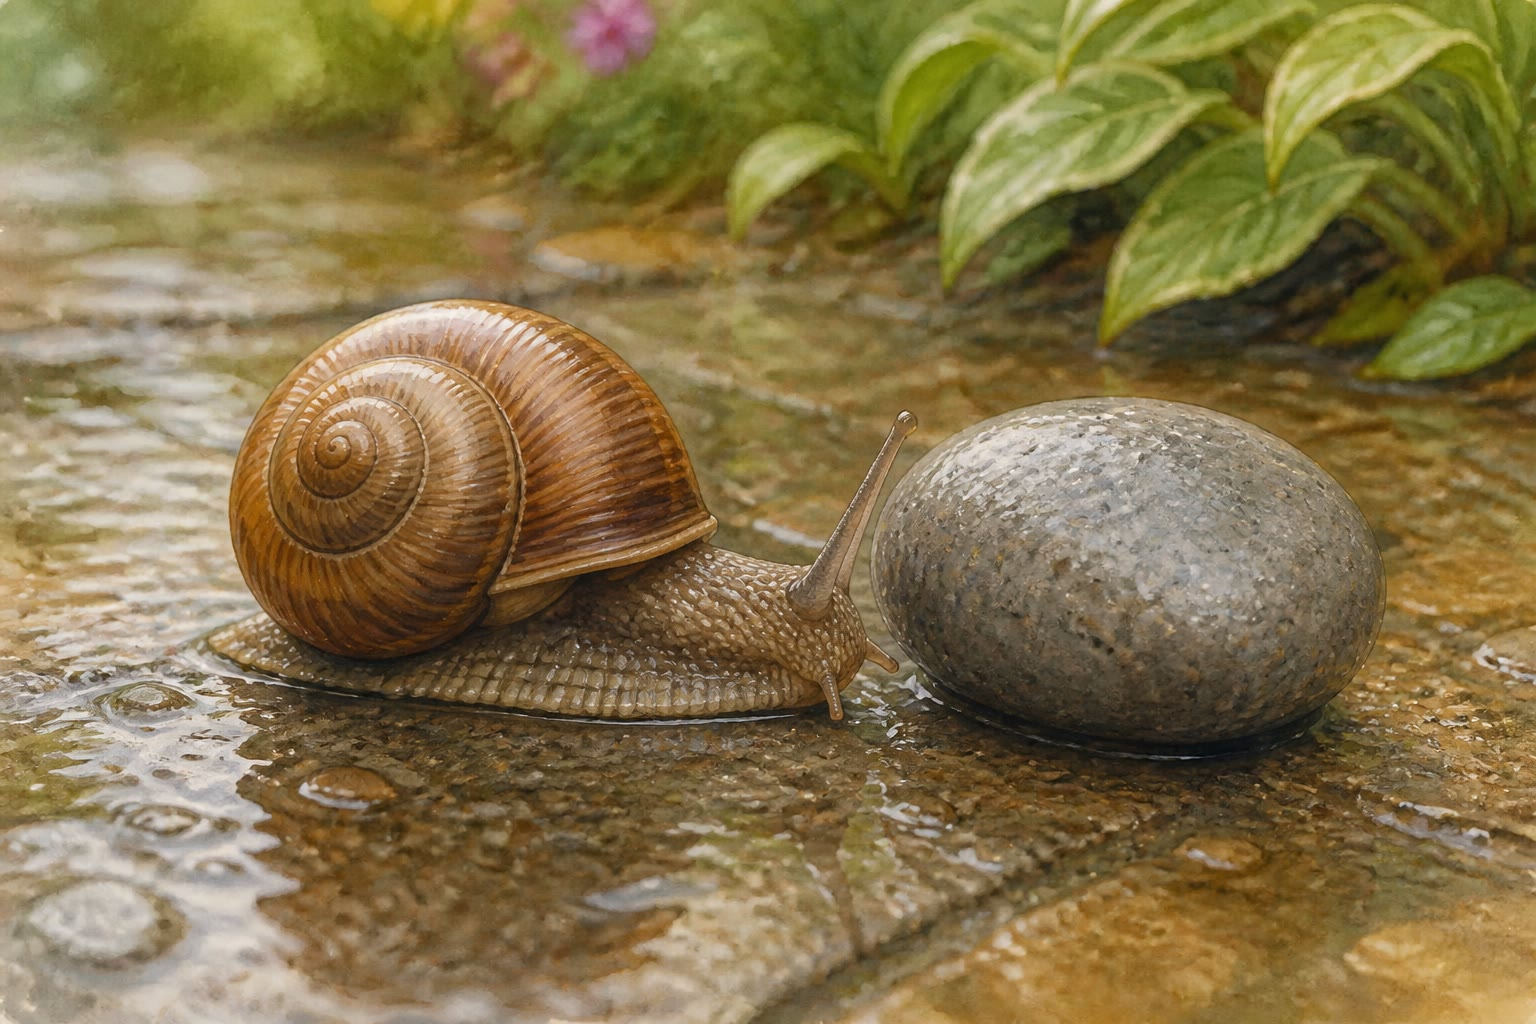
\includegraphics[width=0.62\linewidth]{images/book1/ai/g1-living-snail.jpg}

{\small 本章两位“邻居”的真人版：其中一位正
慢慢地朝某处爬去，它可不是小石子。}
\end{omfigure}

\begin{proposition}[生命的特征]\label{prop:g1:living-or-not:signs}
\omterm{def:g1:living-or-not:living}{生物}具有以下特征：
\begin{enumerate}
  \item 它\emph{出生}\index{出生}过；
  \item 它\emph{取食}\index{取食}——吃进食物，或者像植物
        那样借助光自己制造食物；
  \item 它\emph{生长}\index{生长}；
  \item 它能生宝宝——生出和自己一样的新\omterm{def:g1:living-or-not:living}{生物}；
  \item 它有一天会\emph{死亡}\index{死亡}。
\end{enumerate}
没有这些特征的东西，就不是\omterm{def:g1:living-or-not:living}{生物}。
\end{proposition}
\admitted

\begin{remark}[每一个特征都重要]\label{rem:g1:living-or-not:allsigns}
仅凭一个特征是不够的。汽车会“喝”燃料，冰柱
在冷天里会变长——但汽车是造出来的，不是出生的，
冰柱没有小冰柱。要想是活的，一样东西必须
\emph{同时}具备生命的这些特征：出生、取食、生长、
生出新\omterm{def:g1:living-or-not:living}{生物}、死亡。
\end{remark}

\section{活的、不再有生命、从未有过生命}

\begin{definition}[非生物]\label{def:g1:living-or-not:nonliving}
\emph{非生物}\index{非生物}是指
没有生命的东西。它分为两类：
\begin{itemize}
  \item \emph{从未有过生命}\index{从未有过生命}的东西：
        小石子、水、风、一辆自行车；
  \item \emph{不再有生命}\index{不再有生命}的东西，或\emph{来自}\omterm{def:g1:living-or-not:living}{生物}的东西：地上的一片
        枯叶、一张木桌、一件羊毛套头衫。
\end{itemize}
\end{definition}

\begin{example}[木桌]\label{ex:g1:living-or-not:table}
木桌不取食，也不生长：它不是\omterm{def:g1:living-or-not:living}{生物}。
但它的木头曾经是活的：它来自一棵树，这棵树是从一颗
种子长出来的，生长了许多年，后来被砍倒。这张桌子是\omterm{def:g1:living-or-not:nonliving}{非生物}，
但它来自\omterm{def:g1:living-or-not:living}{生物}。
\end{example}

\begin{example}[机器人呢？]\label{ex:g1:living-or-not:robot}
一个玩具机器人会移动，会发出声音，它的灯光像一只
小眼睛一样一闪一闪。它是活的吗？来检查一下特征：它是在工厂
里造出来的，不是出生的；它的电池不是让它生长的食物，它永远
不会生出小机器人。机器人会动，但它不是\omterm{def:g1:living-or-not:living}{生物}。
\end{example}

\begin{omfigure}
\begin{tikzpicture}
  % three sorting boxes
  \draw[thick, omDef, fill=omDef!6] (0,0) rectangle (3.9,2.6);
  \draw[thick, omProp, fill=omProp!6] (4.3,0) rectangle (8.2,2.6);
  \draw[thick, omExo, fill=omExo!6] (8.6,0) rectangle (12.5,2.6);
  \node[font=\small\bfseries, omDef] at (1.95,2.25) {活的};
  \node[font=\small\bfseries, omProp] at (6.25,2.25) {曾经是活的};
  \node[font=\small\bfseries, omExo] at (10.55,2.25) {从未有过生命};
  \node[font=\small, align=center, text width=3.6cm] at (1.95,1.1)
    {蜗牛 \\ 雏菊 \\ 你！};
  \node[font=\small, align=center, text width=3.6cm] at (6.25,1.1)
    {一片枯叶 \\ 一把木勺 \\ 小路上的一根羽毛};
  \node[font=\small, align=center, text width=3.6cm] at (10.55,1.1)
    {小石子 \\ 小水洼 \\ 玻璃弹珠};
\end{tikzpicture}

{\small 用三个盒子给世界分类：活的、\omterm{def:g1:living-or-not:nonliving}{不再有生命}的、
\omterm{def:g1:living-or-not:nonliving}{从未有过生命}的。}
\end{omfigure}

\begin{method}[怎样判断：是生物还是非生物？]\label{met:g1:living-or-not:decide}
依次问自己以下关于生命的问题：
\begin{enumerate}
  \item 它出生了吗？它取食吗？它生长吗？
  \item 它能生宝宝吗？它总有一天会死亡吗？
  \item 如果答案都是“是”，它就是\omterm{def:g1:living-or-not:living}{生物}。
  \item 如果答案是“否”，再问一个问题：它是否
        \emph{来自}\omterm{def:g1:living-or-not:living}{生物}，比如树的木头？
\end{enumerate}
\end{method}

\begin{remark}[种子看起来像在睡觉]\label{rem:g1:living-or-not:seed}
一颗干燥的豆子种子装在包装袋里，看起来和鹅卵石一样静止不动。但把它
放在湿棉花上，几天之内就会长出一条小根：种子一直都是活的，
只是在等待。缓慢、安静的\omterm{def:g1:living-or-not:living}{生物}很容易被误认为是\omterm{def:g1:living-or-not:nonliving}{非生物}——
生命的问题能帮助我们
仔细观察。
\end{remark}

\section{练习}

\begin{exercise}[$\star$]\label{exo:g1:living-or-not:1}
说出生命的五个特征。
今天你能看到小猫正在做其中哪些事情？
\end{exercise}

\begin{exercise}[$\star$]\label{exo:g1:living-or-not:2}
判断下列事物是否为\omterm{def:g1:living-or-not:living}{生物}：(a) 蝴蝶；(b) 自行车；(c) 雏菊；
(d) 云。
\end{exercise}

\begin{exercise}[$\star$]\label{exo:g1:living-or-not:3}
一片枯叶躺在小路上。它现在是活的吗？
它曾经是活的吗？它是从哪里来的？
\end{exercise}

\begin{exercise}[$\star$]\label{exo:g1:living-or-not:4}
汤姆说：“河流是活的——你看，它会流动，还会
发出声音！”请用\cref{met:g1:living-or-not:decide}中的问题，
温和地回答他。
\end{exercise}

\begin{exercise}[$\star$]\label{exo:g1:living-or-not:5}
把图中的三个方框分类——\omterm{def:g1:living-or-not:living}{生物}、曾经是\omterm{def:g1:living-or-not:living}{生物}、
从未是\omterm{def:g1:living-or-not:living}{生物}：蜘蛛、毛线袜、雨滴、树上的苹果、
掉落的松果。
\end{exercise}

\begin{exercise}[$\star$]\label{exo:g1:living-or-not:6}
蜡烛的火焰会“吃”掉蜡油，越长越高，
吹灭它时它就“死”了。火焰是\omterm{def:g1:living-or-not:living}{生物}吗？
哪一个生命的问题的答案是“否”？
\end{exercise}

\begin{exercise}[$\star$]\label{exo:g1:living-or-not:7}
说出你卧室里两样来自\omterm{def:g1:living-or-not:living}{生物}的东西，
比如\cref{ex:g1:living-or-not:table}中的木桌。说出
每样东西分别来自哪种\omterm{def:g1:living-or-not:living}{生物}。
\end{exercise}

\begin{exercise}[$\star$]\label{exo:g1:living-or-not:8}
动手试一试：把一颗干豆子放在靠近窗户的湿棉花上，再把一块鹅卵石放在
旁边的另一块湿棉花上。连续一周，每天看一看。
哪一个会发生变化？这说明了什么？
\end{exercise}

\begin{exercise}[$\star\star$]\label{exo:g1:living-or-not:9}
一个玩具机器人和一只蜗牛都在地板上移动。
请给出两个生命的问题，使它们的答案不同。
\end{exercise}

\begin{exercise}[$\star\star$]\label{exo:g1:living-or-not:10}
蘑菇不像动物那样奔跑，也不像大多数
植物那样是绿色的。请结合\cref{prop:g1:living-or-not:signs}中的特征，
解释为什么蘑菇仍然是\omterm{def:g1:living-or-not:living}{生物}。
\end{exercise}
